\chapter{Kokoelmat} \label{Kokoelmat}
Tutkimuksen kohteena on Scalan standardikirjaston kokoelmat versiosta 2.8 versioon 2.12. Standardikirjastossa on toteutus useimmille yleisimmille kokoelmaluokille kuten taulukoille, listoille, joukoille(\code{Set}) ja assosiaatiotauluille(\code{Map}). Scalan kokoelmaluokat ovat paketissa \code{scala.collection}. Muuttumattomat kokoelmat ovat alipaketissa \code{immutable} ja muuttuvat alipaketissa \code{mutable}.
\cite{scalaCollections}

Muuttumattoman kokoelman sisältämät alkiot eivät voi muuttua alustamisen jälkeen. Tämä tarkoittaa ettei alkioiden lisääminen, poistaminen tai uudelleenjärjestäminen ole mahdollista. Kokoelman muuttamista muistuttavat operaatiot, kuten \code{map}, \code{reverse}, \\\code{fold} ja kokoelmien yhdistäminen, palauttavat aina uuden kokoelman jättäen alkuperäisen kokoelman ennalleen. Käytännössä kuitenkaan aina ei kaikkia muuttumattoman kokoelman alkioita ei tarvitse kopioida, vaan tietorakenteet pyrkivät käyttämään hyväkseen rakenteellista jakamista parantaakseen suorituskykyä ja optimoidakseen muistinkäyttöä. Muuttuvissa kokoelmissa on nimensä mukaisesti mahdollista vaihtaa alkioiden järjestystä, lisätä ja poistaa alkioita kokoelmasta luomatta uutta kokoelmaa.
\cite{scalaCollections}
\cite[Luku 22]{prorgrammingInScala3rd}

Kokoelmaluokat noudattavat piirreluokkien määrittelemää hierarkiaa, joka on paketissa \code{scala.collection}. Hierarkia on sama sekä muuttumattomille että muuttuville kokoelmille. Ylimpänä hierarkiassa on \code{Traverable}-piirreluokka, jolla on yksi välitön aliluokka, \code{Iterable}. \code{Iterable}:lla on kolme välitöntä aliluokkaa \code{Seq}, \code{Set} ja \code{Map}, jotka edustavat järjestyksellisiä kokoelmia, joukkoja ja assosiaatiotauluja. Kuvassa \ref{kokoelmahierarkia} näytetään lisäksi vielä muutama aliluokka.
\cite{scalaCollections}
\begin{figure}[h]
    \centering\usetikzlibrary{shapes.geometric, arrows}


\tikzstyle{trait} = [rectangle, rounded corners, minimum width=2cm, minimum height=1cm,text centered, draw=black, fill=white]
\tikzstyle{arrow} = [thick,->,>=stealth]

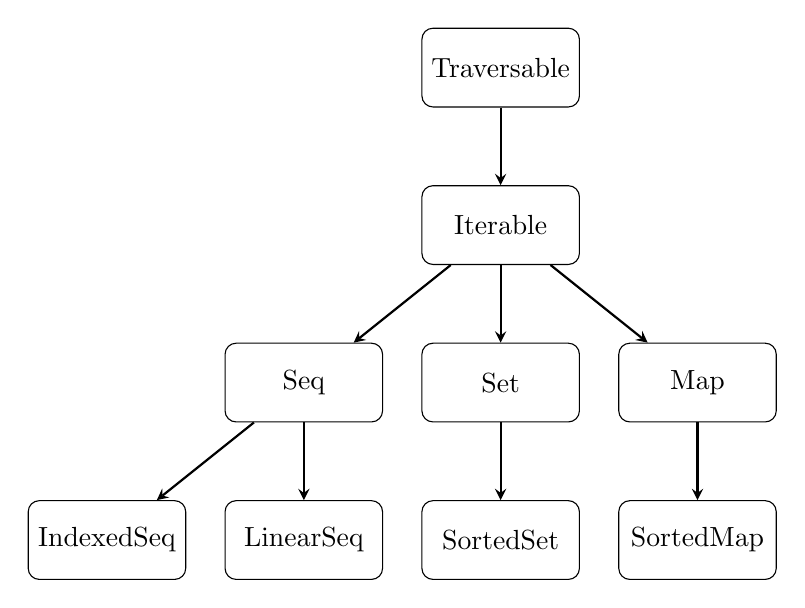
\begin{tikzpicture}[align=center, node distance=2cm]
    \node (traversable) [trait] {Traversable};
    \node (iterable) [trait, below of=traversable] {Iterable};
    \node (set) [trait, below of=iterable] {Set};
    \node (sortedset) [trait, below of=set] {SortedSet};

    \begin{scope}[node distance=25mm]
        \node (seq) [trait, left of=set] {Seq};
        \node (linearseq) [trait, left of=sortedset] {LinearSeq};
        
        \node (map) [trait, right of=set] {Map};
        \node (sortedmap) [trait, right of=sortedset] {SortedMap};
        
        \node (indexedseq) [trait, left of=linearseq] {IndexedSeq};
    \end{scope}

    \draw [arrow] (traversable) -- (iterable);
    \draw [arrow] (iterable) -- (set);
    \draw [arrow] (iterable) -- (seq);
    \draw [arrow] (iterable) -- (map);
    \draw [arrow] (seq) -- (indexedseq);
    \draw [arrow] (seq) -- (linearseq);
    \draw [arrow] (set) -- (sortedset);
    \draw [arrow] (map) -- (sortedmap);

\end{tikzpicture}
    \caption{Kokoelmien hierarkia}\label{kokoelmahierarkia}
\end{figure}


\section{Järjestykselliset kokoelmat}
\todo{Etsi parempi ilmaus järjestykselliselle}
Suorituskykyvertailuun valittiin muuttumattomista kokoelmista \code{List}, joka tyypillinen rekursiivinen linkitetty rakenne funktionaaliessa ohjelmoinnissa, ja \code{Vector}, jossa alkion haku indeksin mukaan on tehokkaampaa. Muuttuvista kokoelmista valittiin \code{Array}, joka on kiinteän kokoinen taulukko, \code{ArrayBuffer}, joka on dynaamisesti kasvava taulukko ja \code{ListBuffer}, joka on dynaamisesti kasvava linkitetty rakenne. Kaikki kyseiset muuttuvat tietorakenteet ovat tyypillisiä olio-ohjelmoinnissa käytettyjä tietorakenteita.

\code{List} on abstrakti luokka, joka kuvaa yhteen suuntaan linkitettyä rekursiivista muuttumatonta listaa, jolla on kaksi konkreettista toteutusta: \code{::} ja \code{Nil}. Epätyhjää listaa kuvaavassa luokassa \code{::}, on kaksi jäsentä: alkio, jota kutsutaan listan \textit{pääksi}, ja \textit{häntä} joka kuvaa listan muita alkioita. Tyhjää listaa ja listan loppumista kuvaa singleton-olio \code{Nil}. Esimerkiksi luvut 1 ja 2 sisältävä lista voidaan ilmaista näin: \code{1 :: 2 :: Nil}. Listan \code{head}-ja \code{tail}-operaatiot sekä listan alkuun lisääminen tapahtuu vakioajassa. Aikakompleksisuus alkion hakemiselle indeksin perusteella on lineaarinen.
\cite{scalaAPI}
\cite{scalaCollections}

\code{Vector} on taulukon ominaisuuksia jäljittelevä muuttumaton tietorakenne, joka on toteutettu puurakenteena, jonka solmut ovat korkeintaan 32-alkioisia taulukoita. Lehtisolmujen taulukot sisältävät vektorin varsinaisia alkioita, ja muut solmut sisältävät alemman tason taulukoita. Jos esimerkiksi alustetaan uusi 70-alkioinen vektori, on se kolmen taulukon puu jossa juurisolmuna olevalla taulukolla on kolme lapsitaulukkoa, joista kahdessa on 32 alkiota ja yhdessä 6 alkiota. Tämä mahdollistaa taulukoiden rakenteellisen jakamisen eri vektori-instanssien kesken, joka vähentää kopioimista ja muistinkäyttöä. Satunnaisten haku-, muokkaus- ja poisto-operaatioiden aikakompleksisuus on log(32, N), eli operaatioiden voidaan ajatella tapahtuvan lähes vakioajassa.
\cite{scalaCollections}
\cite[Luku 4]{highPerformanceProgramming}

\code{Array} on Scalassa erityinen kokoelma, joka mahdollistaa primitiivityyppisten-, \\viittaustyyppisten- ja geneeristen alkioiden tallentamisen. Primitiivityyppisiä alkioita käsitellään ilman alkioiden käärimistä olioiksi. Esimerkiksi kokonaislukuja sisältävä \\\code{Array[Int]} käänntyy Javan \code{int[]}-taulukoksi. Kuten Javassa, taulukon koko ei voi muuttaa alustamisen jälkeen. Verrattuna Javan taulukoihin, \code{Array} tarjoaa kuitenkin huomattavasti enemmän operaatioita. Haku-ja muokkausoperaatiot tapahtuvat vakioajassa. Häntäoperaatio vie kuitenkin lineaarisen ajan, sillä jokainen alkio, poislukien ensimmäinen, joudutaan kopioimaan uuteen taulukkoon.
\cite{scalaCollections}

\code{ArrayBuffer} on dynaamisesti kasvava listarakenne, joka käyttää alkioiden tallentamiseen taulukkoa. Tästä johtuen useimmat operaatiot vastaavat aikakompleksisuudeltaan \code{Array}:ta. Lisäksi \code{ArrayBuffer} mahdollistaa alkion lisäämisen taulukon alkuun, loppuun sekä keskelle. Alkuun ja keskelle lisäämisen aikakompleksisuus on lineaarinen. Muut operaatiot tapahtuvat pääasiassa vakioajassa, poislukien täyteen taulukkoon lisääminen, joka vie lineaarisen ajan.
\cite{scalaCollections}

\code{ListBuffer} on dynaamisesti kasvava muuttuva kokoelma joka on toteutettu linkitettynä rakenteena. Poiketen \code{List}:stä, \code{ListBuffer} mahdollistaa alkioiden lisäämisen rakenteen alkuun ja loppuun vakioajassa. Satunnaisen alkion haku-ja muokkausoperaatiot, sekä rakenteen keskelle lisääminen ovat aikakompleksisuudeltaan lineaarisia. Myös häntäoperaatio vie lineaarisen ajan, sillä kaikki hännän alkiot täytyy kopioida uuteen tietorakenteeseen.   
\cite{scalaCollections}


\section{Joukot ja assosiaatiotaulut}
\todo{Tarkastellaanko ollenkaan?}


\section{Suorituskykyvertailut}

Tutkielmassa on käytetty kokoelmien suorituskykymittauksia on kahdesta eri lähteestä: Li Haoyi:n\cite{haoyiBenchmark} ja Toby Hobsonin\cite{hobsonBenchmark} mittauksista. Haoyin mittauksissa mitataan aikaa, joka operaatioiden suorittamisessa kestää, eli pienempi arvo tarkoittaa parempaa suorituskykyä. Hobsonin mittauksissa tarkastellaan operaatioiden määrää sekunnissa, jolloin suuri luku takoirttaa parempaa suorituskykyä. Hayoin mittauksissa suorituskykyä on mitattu eri kokoisilla kokoelmilla. Kaavioihin on valittu kyseisen operaation kannalta mielekkäät koot kokoelmille.

Järjestyksellisten kokoelmien tapauksessa kiinnostuksen kohteena on yleisimpien operaatioiden suorituskyky: kokoelman luominen, iterointi, alkion satunnainen haku sekä lisääminen ja häntäoperaatio.

Imperatiivisissa kielissä iterointia tehdään yleensä silmukoiden, tavallisesti \code{for} ja \code{while}, avulla. Funktionaalinen paradigma ei kuitenkaan tunne silmukoita ja iterointia tehdään tavallisesti korkeamman asteen funktioiden, kuten \code{map} ja \code{foreach}, avulla.
\cite[Luku 2]{prorgrammingInScala3rd}
Seuraavaksi esitellään molemmat tavat tulostamalla listan parilliset luvut kahdella kerrottuna:
\begin{figure}[h]
    \begin{lstlisting}
        val list = List.range(1, 11)

        // Imperatiivisesti
        for(i <- list)
            if (i % 2 == 0) println(i*2)

        // Funktionaalisesti
        list.filter(_ % 2 == 0).map(_ * 2).foreach(println)
    \end{lstlisting}
    \caption{Iterointi imperatiivisesti ja funktionaalisesti}\label{iterointi_esim}
\end{figure}

\begin{figure}
    \centering
    \pgfplotstableread{
    size    List    Vector  Array
    4096    14100   16200   14200
    16192   55000   62000   55600
    65536   231000  256000  228000
    262144  920000  1030000 910000
}\haoyi

\pgfplotstableread{
    collection  result
    List        396586
    Vector      402363
    Array       321700
    ArrayBuffer 1226833
    ListBuffer  412568
}\hobson

\begin{tikzpicture}
    \begin{axis}[
        width=0.55*\textwidth,
        xshift=-2cm,
        xtick=data,
        xticklabels from table={\haoyi}{size},
        ymin=0,
        name={haoyi},
        title={Haoyi},
        xlabel={Kokoelman koko},
        legend pos=north west,
        legend style={draw=none},
    ]

    \addplot+[blue] table [y=List, x expr=\coordindex]{\haoyi};
    \addplot+[red] table [y=Vector, x expr=\coordindex]{\haoyi};
    \addplot+[green] table [y=Array, x expr=\coordindex]{\haoyi};

    \legend{List, Vector, Array, ArrayBuffer}

    \end{axis}

    \begin{axis}[
        at={(haoyi.south east)},
        xshift=1cm,
        width=0.55*\textwidth,
        ybar,
        ymin=0,
        xtick=data,
        xticklabel style={rotate=45, anchor=north east},
        title={Hobson},
        symbolic x coords={List, Vector, Array, ArrayBuffer, ListBuffer},
        nodes near coords,
        every node near coord/.append style={
            /pgf/number format/fixed,
            font=\scriptsize
        },
    ]
    
    \addplot table[x=collection, y=result]{\hobson};

\end{axis}

\end{tikzpicture}
    \caption{Iterointi}\label{iterointi_kaavio}
\end{figure}

\begin{figure}
    \centering
    \pgfplotstableread{
    collection  result
    List        313253
    Vector      62082283
    Array       60777210
    ArrayBuffer 72734680
    ListBuffer  1107126
}\hobson

\begin{tikzpicture}
    \begin{axis}[
        at={(haoyi.south east)},
        ybar,
        width=12cm,
        height=9cm,
        ymin=0,
        xtick=data,
        title={Hobson},
        symbolic x coords={List, Vector, Array, ArrayBuffer, ListBuffer}
    ]
    
    \addplot table[x=collection, y=result]{\hobson};

\end{axis}

\end{tikzpicture}
    \caption{Satunnainen haku}\label{satunnainenHaku_kaavio}
\end{figure}

\begin{figure}
    \centering
    \pgfplotstableread{
    size    List::  Vector:+    Array:+ Array-prealloc  ArrayBuffer
    64      301     1730        1460    186             691
    1024    4900    28600       260000  2710            10840
    4096    19800   324000      3170000 11000           43000
}\haoyi

\begin{tikzpicture}
    \begin{axis}[
        width=12cm,
        height=9cm,
        xtick=data,
        xticklabels from table={\haoyi}{size},
        ymin=0,
        ymax=55000,
        name={haoyi},
        title={Haoyi},
        xlabel={Kokoelman koko},
        legend pos=north west,
        legend style={draw=none},
    ]

    \addplot+[blue] table [y=List::, x expr=\coordindex]{\haoyi};
    \addplot+[red] table [y=Vector:+, x expr=\coordindex]{\haoyi};
    \addplot+[green] table [y=Array:+, x expr=\coordindex]{\haoyi};
    \addplot+[black] table [y=Array-prealloc, x expr=\coordindex]{\haoyi};
    \addplot+[yellow] table [y=ArrayBuffer, x expr=\coordindex]{\haoyi};

    \legend{List::, Vector:+, Array:+, Array-prealloc, ArrayBuffer}

    \end{axis}

\end{tikzpicture}
    \caption{Kokoelman luominen}\label{kokoelmanLuominen_kaavio}
\end{figure}

\begin{figure}
    \centering
    \pgfplotstableread{
    collection              result
    List                    307
    List(prepend)           39799
    Vector                  26882
    Array                   49790
    ArrayBuffer             173677
    ListBuffer              69692
    ListBuffer(prepend)     39799
}\hobson

% "As you can see in the source, I actually allocated a 1000 element array then copied each element into the slot so it’s not strictly an append operation."

\begin{tikzpicture}
    \begin{axis}[
        at={(haoyi.south east)},
        ybar,
        width=12cm,
        height=9cm,
        ymin=0,
        xtick=data,
        title={Hobson},
        ylabel={ops/s},
        symbolic x coords={List, List(prepend), Vector, Array, ArrayBuffer, ListBuffer, ListBuffer(prepend)},
        nodes near coords,
        every node near coord/.append style={/pgf/number format/fixed},
        xticklabel style={rotate=45, anchor=north east},
    ]
    
    \addplot table[x=collection, y=result]{\hobson};

\end{axis}

\end{tikzpicture}
    \caption{Kokoelman loppuun lisääminen}\label{kokoelmanLoppuunLisaaminen_kaavio}
\end{figure}

\begin{figure}
    \centering
    \definecolor{list}{HTML}{4F81BD}
\definecolor{vector}{HTML}{C0504D}
\definecolor{array}{HTML}{00FF00}
\definecolor{arraybuffer}{HTML}{9F4C7C}
\definecolor{listbuffer}{HTML}{FCBA03}

\pgfplotstableread{
    size    List    Vector      Array       ArrayBuffer
    16      21      425         582         43
    64      100     1970        4517        166
    256     420     11800       55500       630
}\haoyi

\begin{tikzpicture}
    \begin{axis}[
        width=12cm,
        height=9cm,
        xtick=data,
        xticklabels from table={\haoyi}{size},
        ymin=0,
        name={haoyi},
        title={Haoyi},
        xlabel={Kokoelman koko},
        legend pos=north west,
        legend style={draw=none},
    ]

    \addplot+[blue] table [y=List, x expr=\coordindex]{\haoyi};
    \addplot+[red] table [y=Vector, x expr=\coordindex]{\haoyi};
    \addplot+[green] table [y=Array, x expr=\coordindex]{\haoyi};
    \addplot+[yellow] table [y=ArrayBuffer, x expr=\coordindex]{\haoyi};

    \legend{List, Vector, Array, ArrayBuffer}
\end{axis}
\end{tikzpicture}
    \caption{Häntäoperaatio}\label{hantaoperaatio_kaavio}
\end{figure}

\todo{Laiskat kokoelmat?}
